\chapter{Development and Implementation}
\label{cha:implementation}
\chapterquote{It's done, when it's done}{An English Phrase}
The sections in this chapter will describe the various stages of development and implementation of this Bachelor thesis' application. At first the basic idea of the layout and the individual views will be described and explained. To get an even better impression the early paper prototype will be shown. Afterwards a short description of the aspired time schedule for the development as well as the creation of the written elaboration is given.

The implementation of the basic layout which was displayed and explained with the help of the paper prototype, will be the first part describing the actual implementation process.
Second, the handling of the data to be visualized is explained. This covers the server based access as well as local storing and loading. 

After the preparations for the visualization have been set forth, the different views will be described. Starting with the explanation of the map view, it will be clarified how the loaded data is visualized. This is followed by the section focusing on the chart view. It explains how a library is used to draw pie charts and how the loaded data has to be prepared. The last section describes how the timeline was implemented. It covers, how one can draw its own views in Android and how to make use of gestures.
\newpage
\section{Paper Prototype}
\label{sec:paper_prototype}
The first step of the development process was the creation of a paper prototype. It was needed to demonstrate the idea and visual appearance of the project and application. Another advantage of the paper prototype is to be able to show different people the application and get feedback without even writing one line of code. This provides the ability to eliminate possible false estimations  in the forefront of the application's implementation. False estimations may be the assumption of wrong needs of possible future users or the creation of an non intuitive layout. In the following the paper prototype will be shown and explained. Any changes to the paper prototype will be discussed in the respective section of this chapter. 

The\mnote{Basic layout} first idea was to split the screen into two parts, an option part and a view part. The left part should be the option part, occupying one sixth of the visible screen. It should always display the following, in appearing order listed, options.\\
In the top left a view selection containing three buttons  ordered vertically with titles ``MapView'', ``ChartView'' and ``Timeline'' are displayed. Taping one of those buttons causes a view switch to display the respective view.\\
Under the view selection a list of options should be visible. Those options vary from view to view but should always contain a button at the top of the list displaying the currently selected date. Tapping on this button causes a date-selection-window to pop up. Selecting a date leads to an update of the displayed view, now visualizing the respective data.
Other options will be explained together with their respective views.

When \mnote{MapView} the application has been loaded, the user will be displayed the map view thus making it the application's start view. The view will display a map with a route, representing the user's visited locations. On start up the selected date will be the current day and therefor the draw route represents the user's latest movements. Tapping on the route should bring up a speech bubble which contains information about the tapped location. Those informations will be the time spend on that location, the used applications and possibly shot photos.\\
The view provides two special options. The first option is represented by a check box and has the title ``Photos''. The option provides the ability to highlight those locations, where a photo was taken. The second option is called ``Apps''. It lets the user pick applications from a list and colors all parts of the route where those specified applications were used. Those options would provide a great tool to quickly get an overview over the position data of specific applications and actions. 

\begin{figure}[h]
%\begin{minipage}[c][\textheight]{\textwidth}
	\caption{Map-View, click on road}
	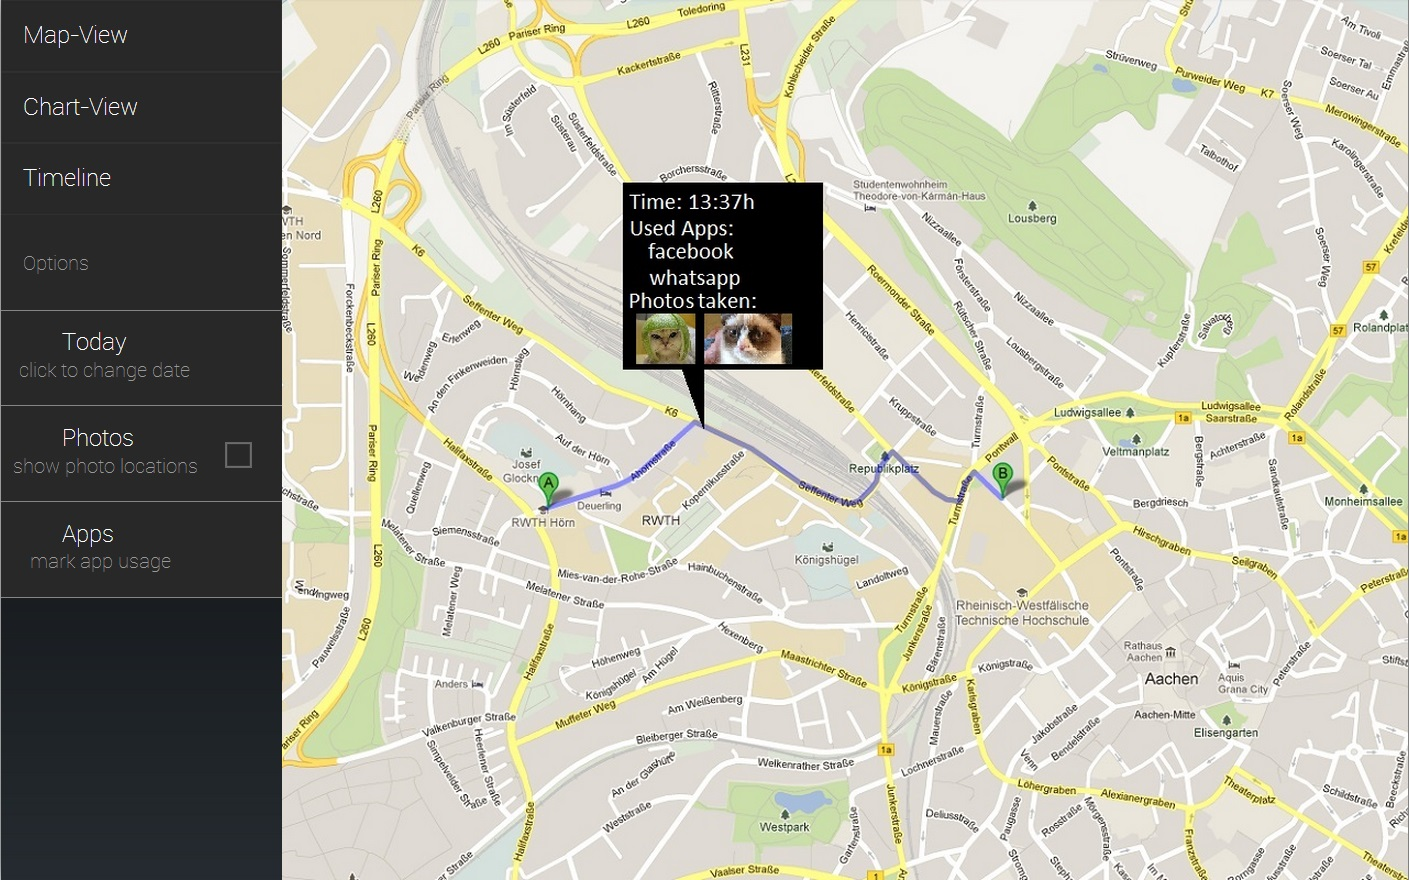
\includegraphics[width=\textwidth]{images/Design/1b_onClickPageView.jpg}
%\end{minipage}
\end{figure}

The second view, the chart view, shows the user his or hers daily activities in form of a pie chart.

\begin{figure}[h]
%\begin{minipage}[c][\textheight]{\textwidth}
	\caption{Chart-View}
	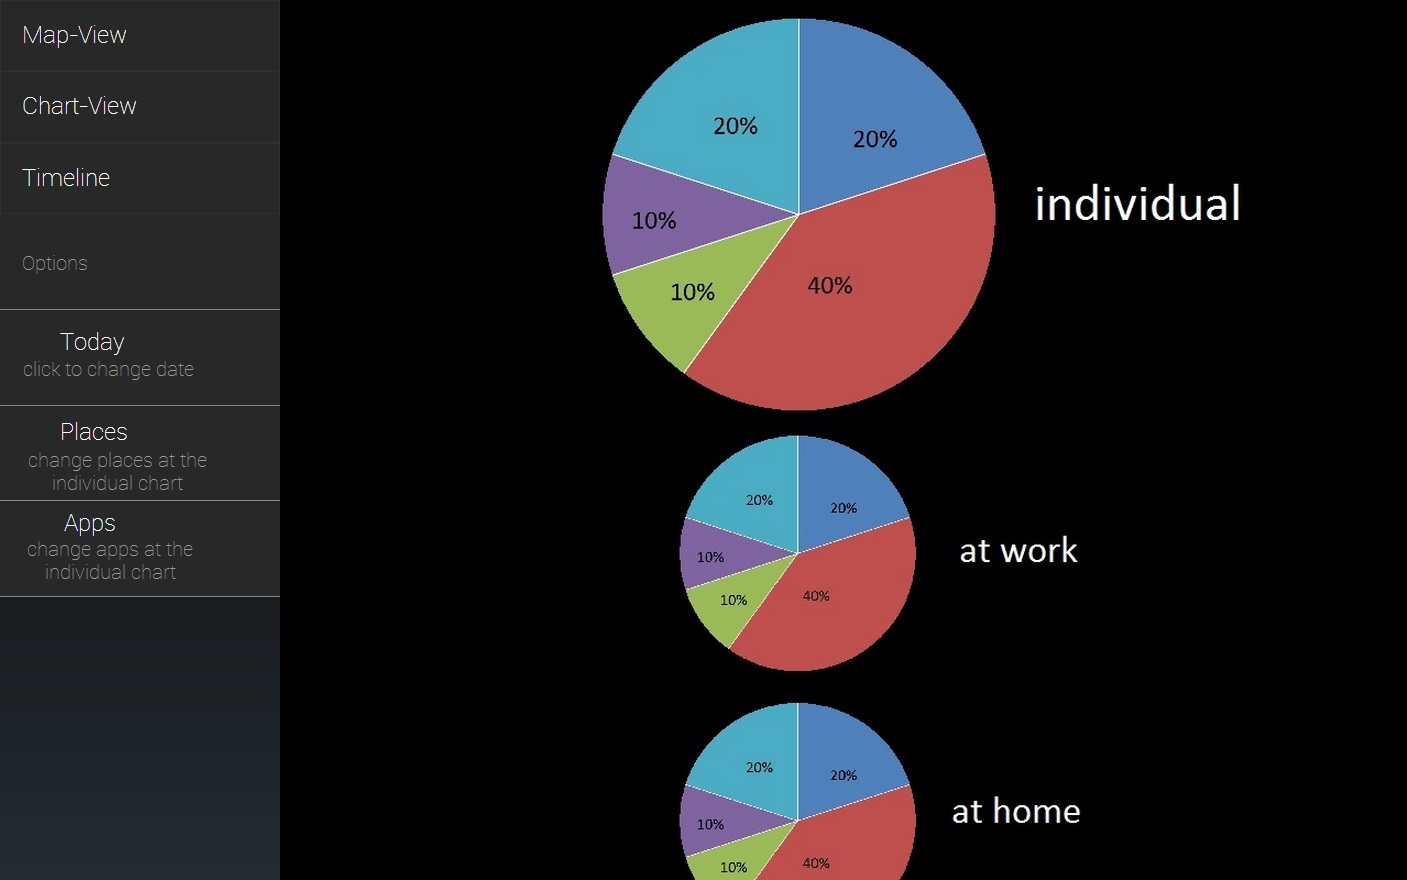
\includegraphics[width=\textwidth]{images/Design/2_ChartView.jpg}
%\end{minipage}
\end{figure}

\begin{figure}[h]
%\begin{minipage}[c][\textheight]{\textwidth}
	\caption{Timeline}
	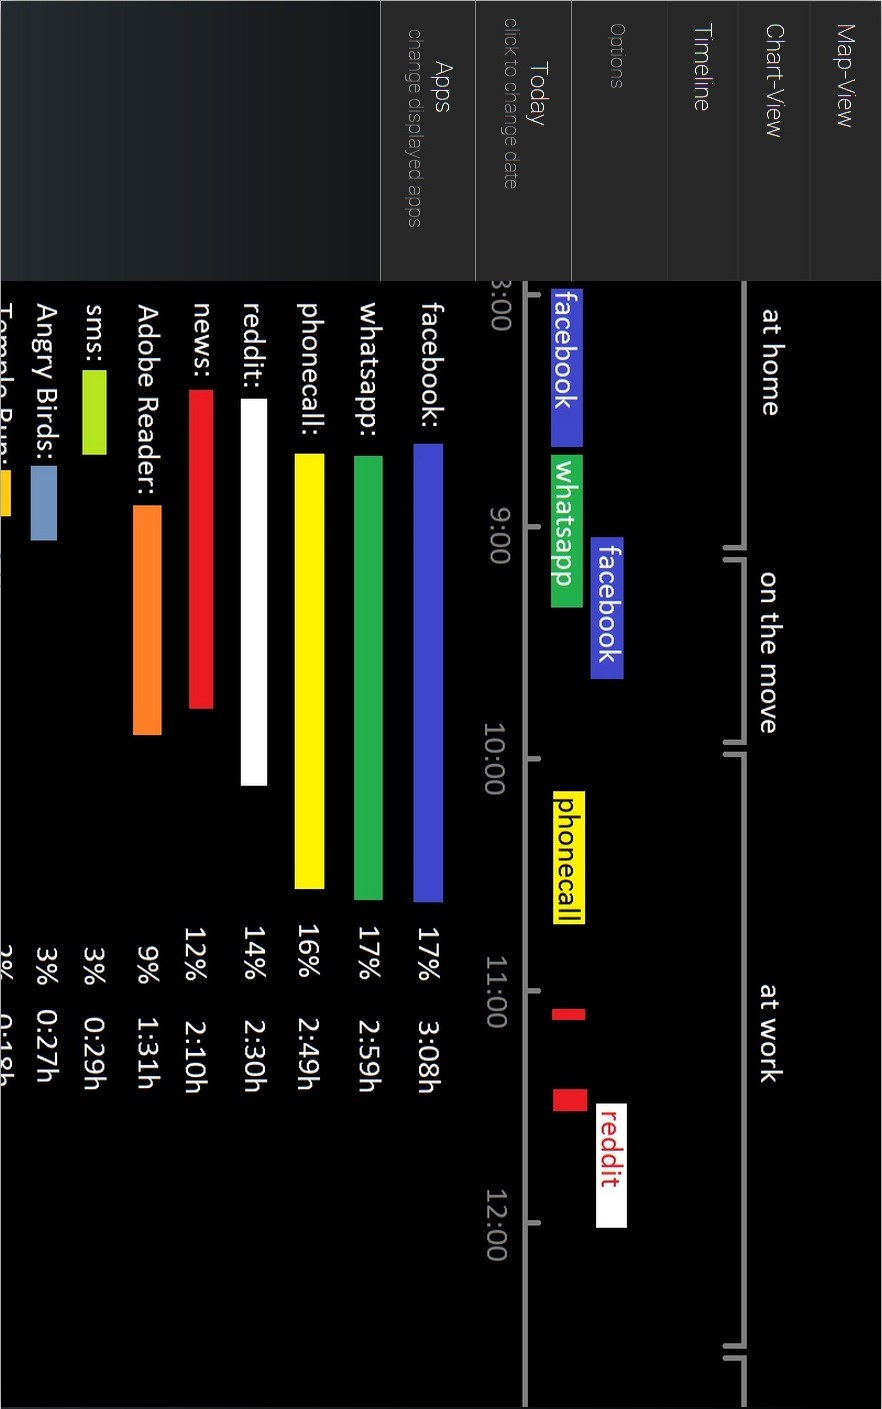
\includegraphics[width=\textwidth]{images/Design/3_TimeLine.jpg}
%\end{minipage}
\end{figure}

\newpage
\section{Time Schedule}
\label{subsec:time_schedule}

\newpage
\section{Basic Layout}

\newpage
\section{Data Management}

\newpage
\section{Mapview}

\newpage
\section{Chartview}

\newpage
\section{Timeline}
%
%The WaveLoc API, as described in chapter \ref{cha:waveloc_api}, offers functionalities to handle the information about the users that are stored in the database up to date, to provide data about participants of WaveLoc (users or POIs) that are close by, and it maintains the friends- and favorite-lists of every user.
%
%As \mnote{Transferring the API} already mentioned in section \ref{sec:waveloc_api__functionalities}, this API uses \emph{PHP}, \emph{MySQL} and runs on the web-server \emph{Apache}. It is possible to transfer this system from one server to another one by installing the whole set of files onto the destination server. One only has to adjust some rights, the content of some files, and to set up the database. The scripts have to get write access to the folders \texttt{/smarty/cache}, \texttt{/smarty/configs}, and \texttt{/smarty/templates\_c}. Thus, they have to get the required rights (\texttt{chmod 775}\footnote{Full rights for the root-user and the owner and rights to read/write for every other user}). The only three files that have to be adjusted are the \texttt{.htaccess} in the root directory of the API, the \texttt{/data/config.php}, and  \texttt{/data/server.php}. In the first file, only the domain has to be adjusted:
%
%\begin{lstlisting}
%ErrorDocument 404 http://wave.thues.com/404.htm
%\end{lstlisting}
%
%\pagebreak
%The second file contains six variables concerning the API that determine default values, among others:
%
%\begin{lstlisting}
%<?PHP
%	$mail_admin = "hendrik@thues.com";
%	// the title of the application
%	$appname = "WaveLoc";
%	// time when an inactive user is set offline
%	$idle_time_sec = "300";
%	// default radius
%	$std_radius = "300";
%	// default time to POI
%	$std_timetopoi = "15";
%	// distance of offline-users 
%	$max_distance = "31337000";
%?>
%\end{lstlisting}
